\documentclass[../../dd.tex]{subfiles}

\begin{document}

	\chapter{User Interface Design}

	We have already described all the main interfaces that the application can show on the chapter 3.1.1 of the RASD. In that chapter we have  described also the input and the action that each user can do, and shown a possible graphic layout of the pages using some mock object. In this chapter we will focus on the navigation between this pages and we will describe in a more specific way the input form. To do that we use a UX diagram UML, with which we give a global overview of all the possible pages with the relative forms. 
	
	\begin{figure}[H]
				\centering
				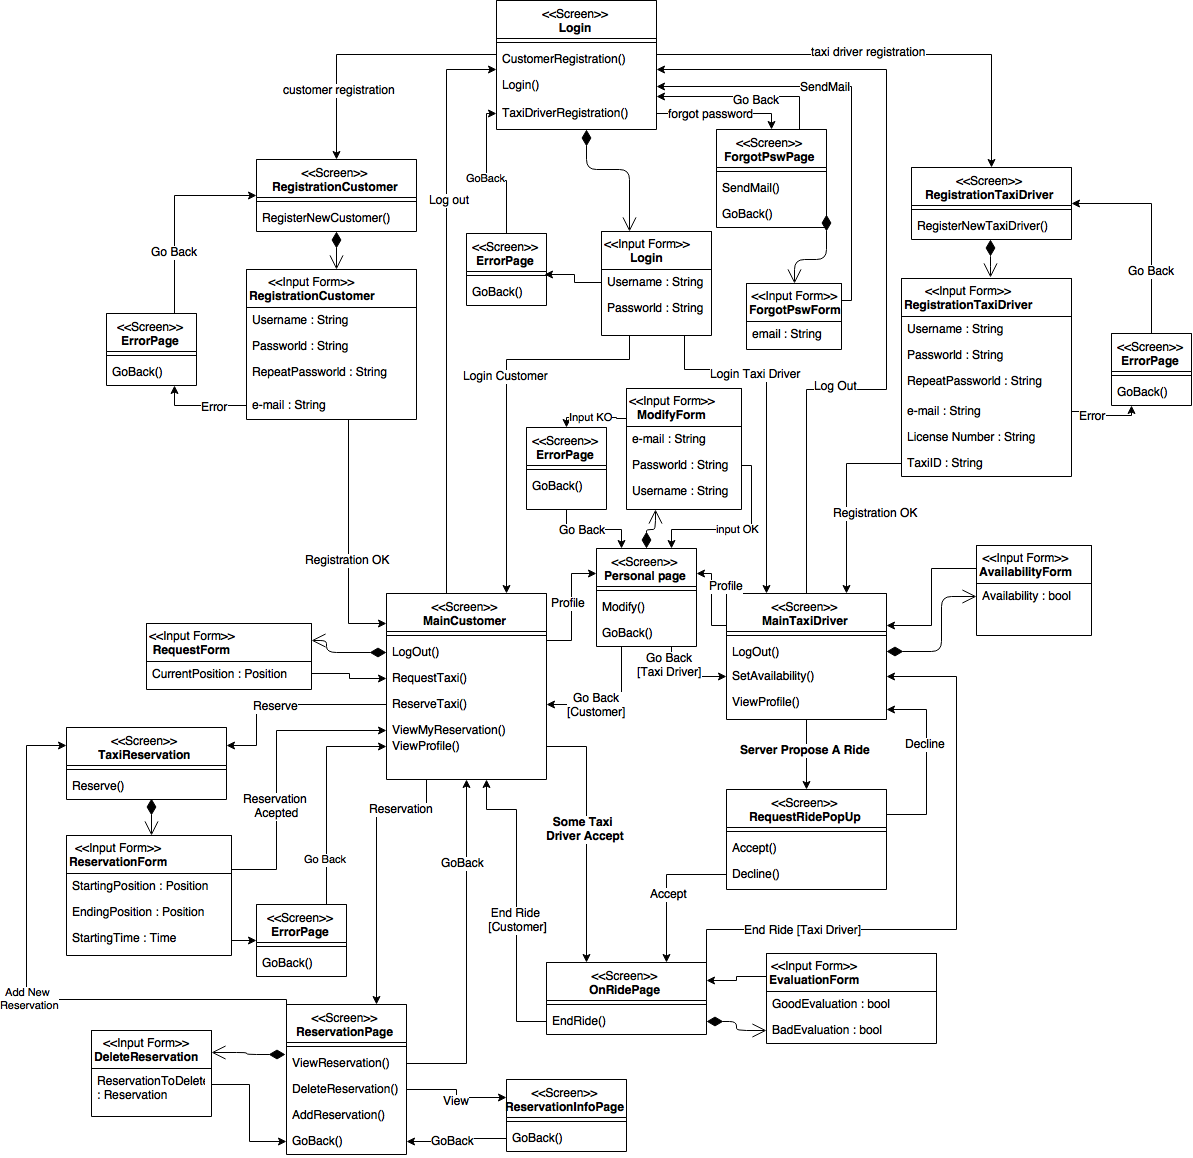
\includegraphics[width=\textwidth, scale=0.5]{../images/UserInterfaces.png}
			\caption{UX Diagram UML}\label{fig:UXDiagram}
		\end{figure}
		
Note: We use [Customer] or [TaxiDriver] on the transition to identify the return page if you are respectively logged as a customer or a taxi driver. We do this because the incoming pages have no differences if you are logged as a customer or as a taxi drivers.
Note: The transitions with the bold text are transitions that do not depend on the input of the user. So, this kind of translations are, for example, pop up that are showed when on the system something has happened. E. g. a taxi driver that is on his main page can pass on the RequestRidePopUp screen without make any move, simply the pop up is shown when the system wants to ask to the taxi driver if he wants to take that ride.

\end{document}